\documentclass{article}
\usepackage{graphicx}
\usepackage{subcaption}
\usepackage[margin=1in]{geometry}
\usepackage{gensymb}

\begin{document}

\begin{figure}[ht]
\centering
\begin{subfigure}{\linewidth}
\centering
\begin{subfigure}{0.45\textwidth}
	\centering
	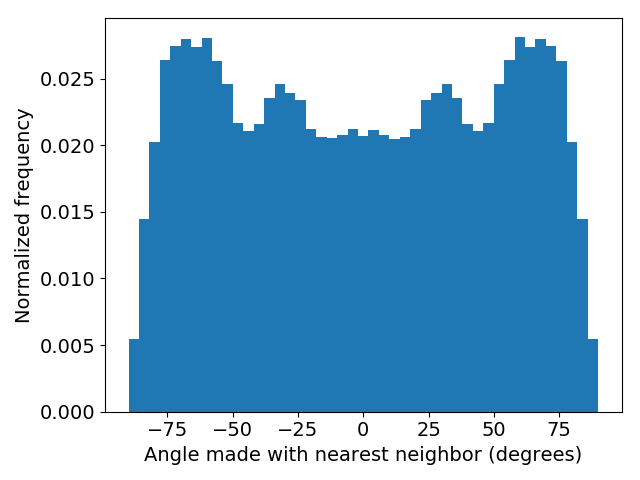
\includegraphics[width=\linewidth]{offset_tail_packing.png}
	\caption{}~\label{fig:offset_tails}	
\end{subfigure}
\begin{subfigure}{0.45\textwidth}
	\centering
	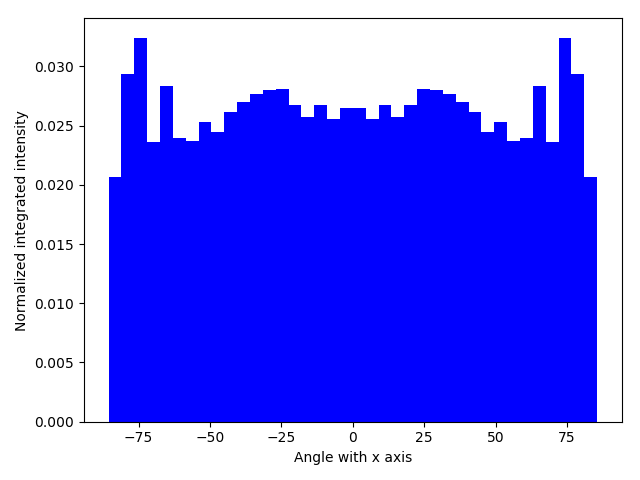
\includegraphics[width=\linewidth]{offset_angle_v_I.png}
	\caption{}~\label{fig:layered_tails}
\end{subfigure}
\end{subfigure}
\begin{subfigure}{\linewidth}
\centering
\begin{subfigure}{0.45\textwidth}
	\centering
	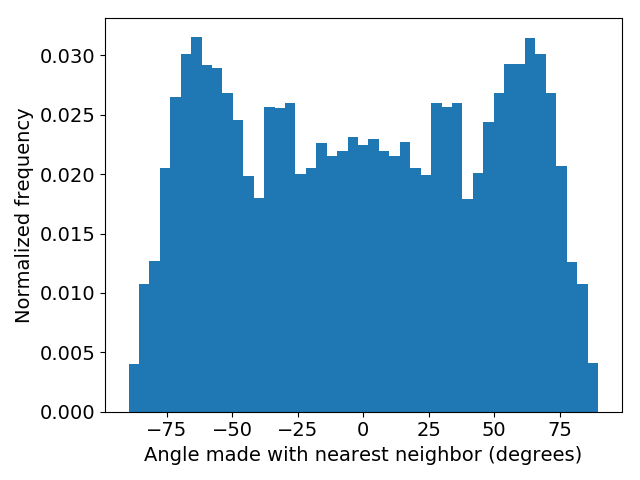
\includegraphics[width=\linewidth]{angles_traj_layered.png}
	\caption{}~\label{fig:rz_layered}
\end{subfigure}
\begin{subfigure}{0.45\textwidth}
	\centering
	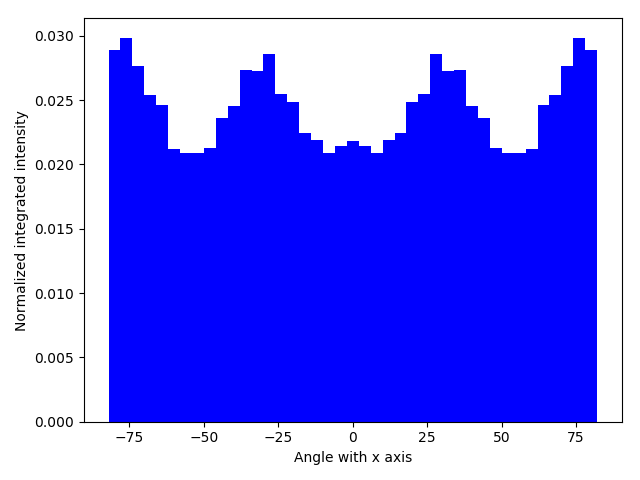
\includegraphics[width=\linewidth]{layered_angle_v_I.png}
	\caption{}~\label{fig:test}
\end{subfigure}
\end{subfigure}
\caption{The distribution of angles w.r.t. the xy plane between alkane chain tail centroids and nearest 
neighbor centroids for equilibrated parallel displaced (a) and sandwiched (c) configurations. The 
same peaks are visible when the 2D simulated diffraction data is radially integrate in the R-alkanes region,
(b) and (d) respectively.}~\label{fig:tail_packing}
\end{figure}

\end{document}
